\subsection{Пошук відповідності між кадрами}

Рух камери не є рідкістю для відеозаписів лекцій. Камера може труситись,
коли її прикріплено до столу, де студенти пишуть лекцію, або від
вібрацій полу, коли викладач ходить по ньому. Камеру може рухати
оператор для того, щоб сфокусувати увагу глядачів на певному сегменті
дошки. У даному розділі описано оцінку гомографії за допомогою
дескриптора ознак SIFT як одного з кроків вирішення вищеописаних
проблем.

Оскільки дошка вважається плоскою поверхнею, побудувати відповідність
між точками дошки на різних зображеннях можна за допомогою гомографії.
Рухи камери під час лекції можуть змінюватися від незначних
субпіксельних зсувів до зміщень, в результаті яких видимою стає частина
дошки, яка до цього була прихованою. Наша мета ~---~ зробити слайди, де
камера виглядає статичною, а сегменти дошки поступово стають видимими та
поєднуються для утворення панорами.

\subsubsection{SIFT}

У 1999 році англієць Девід Лоу представив алгоритм SIFT (scale-invariant feature transform)
\cite{sift} (укр. масштабонезалежне перетворення ознак). Даний алгоритм
застовується для знаходження ключових точок (локальних ознак) (англ. feature points, keypoints) зображення.
Метод досить точно і швидко знаходить дані точки.
Головною перевагою алгоритму є інваріантність щодо просторової орієнтації та якості освітлення.
Має широке застосування в області комп'ютерного зору як один з кроків для побудови 3D-карт,
ректифікації стереопари та виявлення об'єктів.

Ми можемо також використовувати дескриптори ознак, такі як SURF \cite{surf} або ORB \cite{orb},
щоб знайти ключові точки, але був обраний SIFT,
оскільки під час експериментів він надав візуально кращі результати, ніж
інші алгоритми.

Коротко розпишемо структуру алгоритму.

\begin{enumerate}
    \item Пошук масштабно-просторових екстремумів.
          На даному етапі потрібно знайти зони зображення та такі масштаби, які можна повторно
          знайти при різних перспективах (точок погляду). Тут використовується просторове та
          масштабно інваріантне ядро оператора Ґаусса з операцією згортки
          до зображення
          \begin{equation*}
              L(x,y,\sigma) = G(x,y,\sigma) \ast I(x,y),
          \end{equation*}
          де
          \begin{equation*}
              G(x,y,\sigma) = (1/2\pi\sigma^2)\exp({-(x^2+y^2)/2\sigma^2}).
          \end{equation*}
          Будується різниця Ґауссіан (DoG метод) (рис. \ref{fig:swift1}) з константою $k$
          \begin{equation*}
              D(x,y,\sigma) = (L(x,y,k\sigma) - L(x,y,\sigma)).
          \end{equation*}

          Тобто початкове зображення поступово піддається згорткам ґауссіанів з константою
          $k$ на кожну епоху. Причому епохи відрізняється між собою значенням $k = 2^{1/s}$,
          де $s\in\mathbb{N}$ показує на скільки інтервалів розділити кожну епоху.
          В стеку однієї епохи зберігається $s+3$ зображень. Коли епоха завершується,
          створюється нове ґауссове зображення з двох найвищих в стеку
          шляхом взяття кожного 2-го пікселя рядка та колонки.

          \begin{figure}[H]
              \centering
              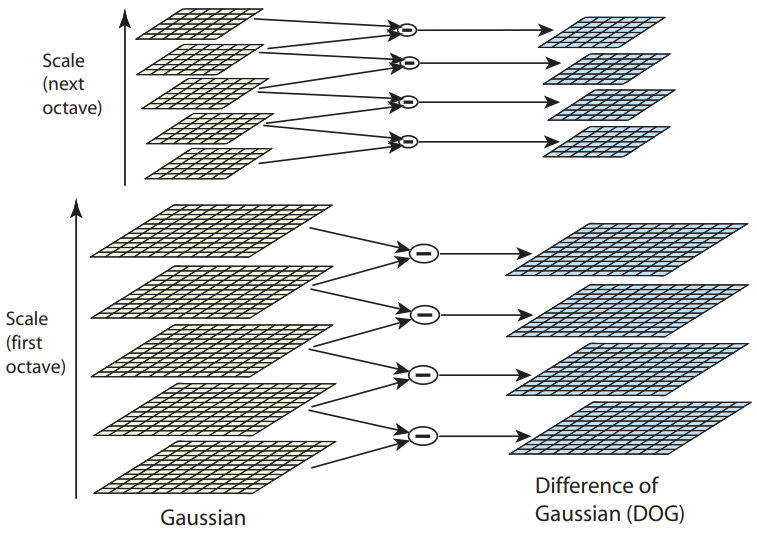
\includegraphics[width=0.5\textwidth]{images/sift1}
              \caption{Знаходження різниць Ґауссіанів 1-ий етап SIFT \cite{sift}
                  \label{fig:swift1}
              }
          \end{figure}

          \subitem Пошук локальних екстремумів. Для знаходження локальних екстремумів
          (рис. \ref{fig:swift2}) зображення
          різниці ґауссіан якоїсь точки беруться 8 сусідів цього ж зображення і 9 зображення
          різниць зверху та знизу. Точка є екстремумом, якщо її значення більше або менше за
          значення всіх її сусідів.

          \begin{figure}[H]
              \centering
              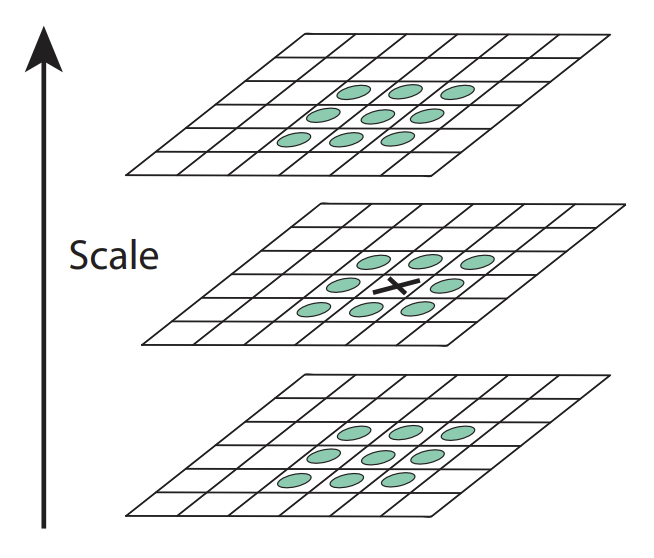
\includegraphics[width=0.3\textwidth]{images/sift2}
              \caption{Пошук локальних екстремумів: 2-ий етап SIFT \cite{sift}
                  \label{fig:swift2}
              }
          \end{figure}

          \subitem Частота вибірки по масштабу. Тут автор обґрунтовує кількість того,
          скільки разів потрібно робити зміну масштабу зображення.
          Експерименти показують (рис. \ref{fig:swift3}),
          що на даному етапі метод дає велику кількість кандидатів екстремумів,
          і що дуже важко обрахувати їх всіх.

          \begin{figure}[H]
              \centering
              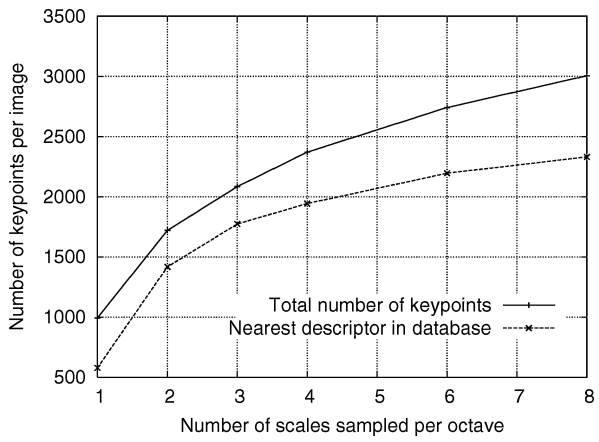
\includegraphics[width=0.4\textwidth]{images/sift3}
              \caption{Графік залежності кількості змін масштабу на кожну епоху до
                  кількості ключових точок на зображенні \cite{sift}
                  \label{fig:swift3}
              }
          \end{figure}
          \subitem Частота вибірки по простору. Пропонується використовувати оптимальне значення
          $\sigma = 1.6$, при якому
          маємо найбільший відсоток збігів екстремумів при багаторазовому повторенні
          експерименту.

    \item Точна локалізація ключових точок. Після знаходження точок-кандидатів потрібно
          відсіяти точки зі слабким контрастом на основі
          інформації про масштаб та відношення головних викривлень. Для цього застосовується розклад
          Тейлора масштабно-просторової функції $D(x,y,\sigma)$ в точці $\boldsymbol{x} = (x,y,\sigma)$.
          \begin{equation}
              D(\boldsymbol{x}) = D + \frac{\partial D^T }{\partial \boldsymbol{x} }\boldsymbol{x} +
              \frac{1}{2}\boldsymbol{x}^T\frac{\partial^2 D}{\partial \boldsymbol{x}^2}\boldsymbol{x}.
              \label{eq:tailor_1}
          \end{equation}
          Місце де знаходиться екстремум $\widehat{\boldsymbol{x}}$,
          \begin{equation}
              \widehat{\boldsymbol{x}} = \frac{\partial^2 D^{-1} }{\partial
                  \boldsymbol{x}^2}\frac{\partial D }{\partial \boldsymbol{x}}.
              \label{eq:extremum}
          \end{equation}
          Підставивши \eqref{eq:extremum} у \eqref{eq:tailor_1}, маємо можливість відсіяти нестабільні
          екстремуми по модулю значення (рис. \eqref{fig:sift45})
          \begin{equation*}
              D(\widehat{\boldsymbol{x}}) = D + \frac{1}{2}\frac{\partial D^{T} }{\partial \boldsymbol{x}}\widehat{\boldsymbol{x}}.
          \end{equation*}

          \begin{figure}[H]
              \centering
              \ContinuedFloat
              \begin{subfigure}[c]{0.3\textwidth}
                  \centering
                  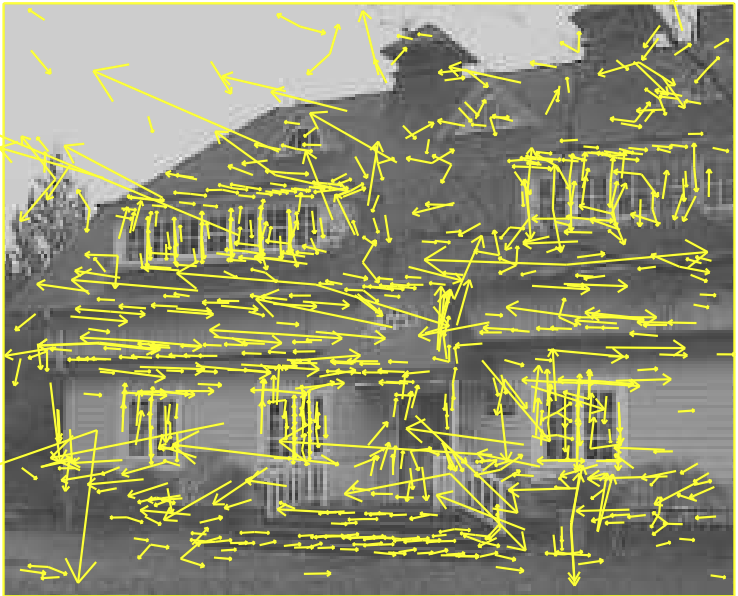
\includegraphics[width=\textwidth]{images/sift4}
                  \caption{ 832 ключових точок
                      \label{fig:swift4}
                  }
              \end{subfigure}
              \begin{subfigure}[c]{0.3\textwidth}
                  \centering
                  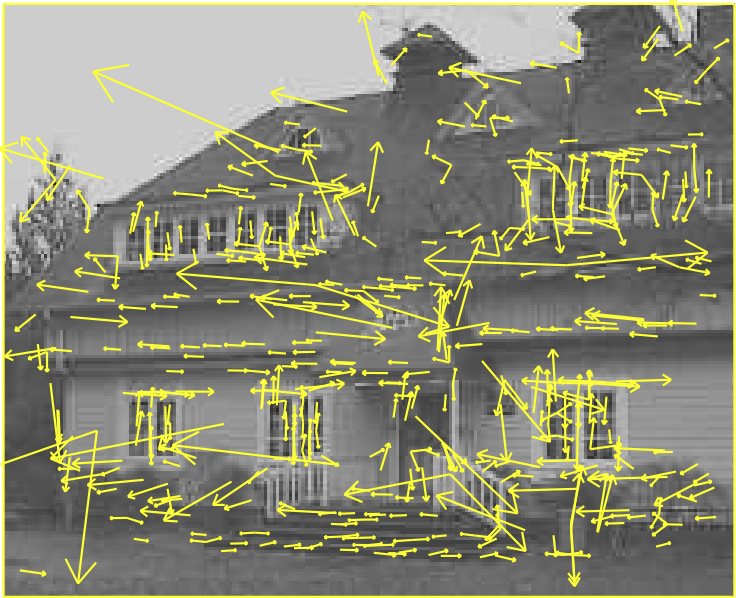
\includegraphics[width=\textwidth]{images/sift5}
                  \caption{ 536 ключових точок
                      \label{fig:swift5}
                  }
              \end{subfigure}
              \caption{Приклад відсіювання екстремумів \cite{sift}
                  \label{fig:sift45}
              }
          \end{figure}
          Таким чином  ми обмежуємо $|D(\widehat{\boldsymbol{x}})| < \alpha$.
          Якщо кожен піксель в діапазоні $[0,1]$, то і
          $ \alpha \in [0,1]$.
    \item Визначення орієнтації градієнтів.
          До кожної точки визначається декілька орієнтацій градієнтів.
          Довжина градієнта по сусідам $m(x,y)$ та його орієнтація $\theta(x,y)$:
          \begin{equation*}
              m(x,y) = \sqrt{(L(x+1,y) - L(x-1,y))^2 + (L(x,y+1) - L(x,y-1))^2},
          \end{equation*}
          \begin{equation*}
              \theta(x,y) = \tan^{-1} (L(x,y+1) - L(x,y-1))/(L(x+1,y) - L(x-1,y)),
          \end{equation*}
          де $L(x,y)$ ~---~ значення згладженого ґауссового зображення з найближчим масштабом.

    \item Дескриптор точок.
          Локальні градієнти обчислюються для кожного масштабу навколо кожної ключової точки.
          На рис. \ref{fig:swift6} наведено створення дескрипторів кожної ключової точки.
          \begin{figure}[H]
              \centering
              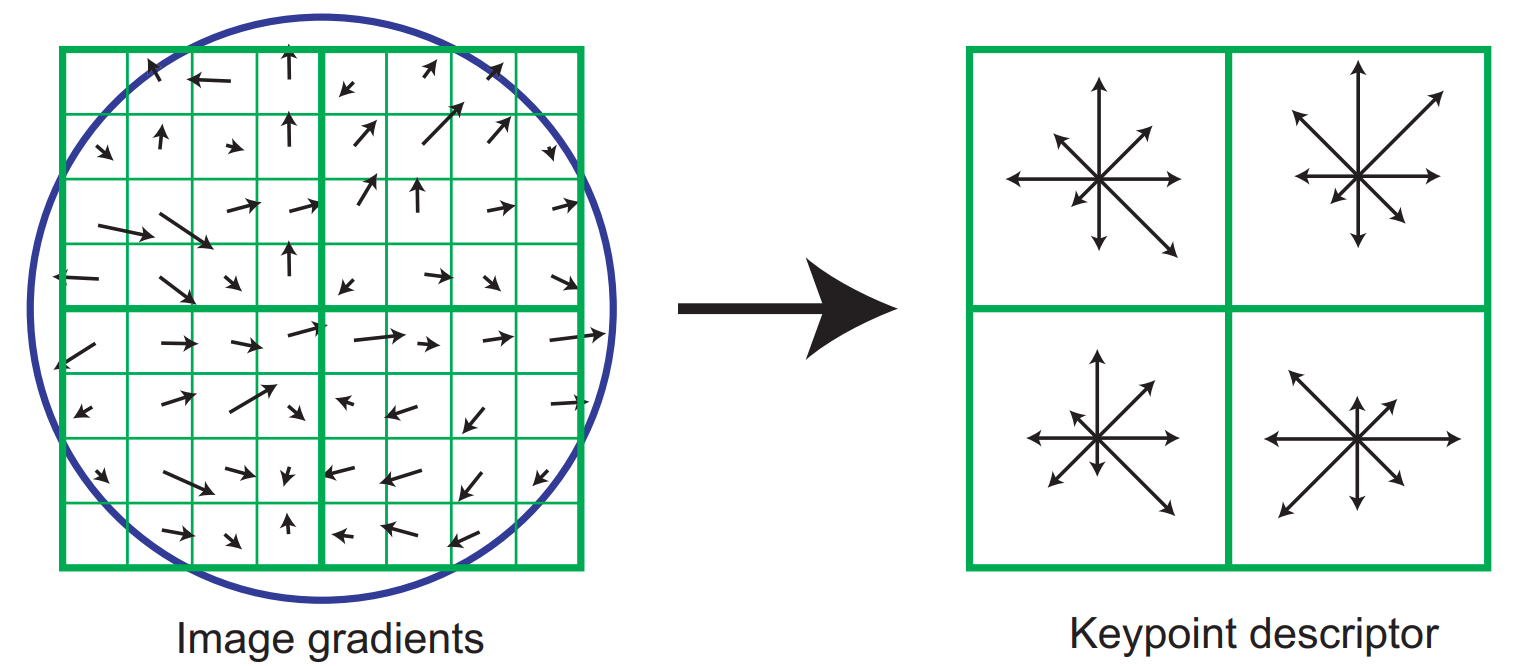
\includegraphics[width=0.5\textwidth]{images/sift6}
              \caption{Створення дескрипторів точок \cite{sift}
                  \label{fig:swift6}
              }
          \end{figure}
\end{enumerate}

\subsubsection{Знаходження відповідних точок зображень}

Дано два кадри \(F^{i}\) та \(F^{i + s}\). Нехай ми маємо набір
\(\left\{ \left( p_{j}^{i},p_{j}^{i + s} \right):j = \overline{1,4} \right\}\)
пар координат відповідних точок, де
\(p_{j}^{i} \in R^{2} \times \left\{ 1 \right\}\) --- координата пікселя
\(p\) на кадрі номер \(i\),
\(p_{j}^{i + s} \in R^{2} \times \left\{ 1 \right\}\) --- відповідна їй
координата на кадрі з номером \(i + s\). Відповідними точками є ті, що є
проекціями однієї і тієї ж точки у просторі.

Нехай $D^i$ та $D^{i+s}$~---~множини дескрипторів кадрів \(F^{i}\) та \(F^{i + s}\)
відповідно. Мета~---~отримати множину \(M^{i,i+s}\) усіх знайдених відповідних точок  між кадрами
\(F^{i}\) і \(F^{i + s}\).
Повний перебір (англ. brute force matcher) (алгоритм \ref{al:brute-force-matcher})
був використаний для знаходження відповідних точок.

\begin{algorithm}[H]
    \caption{Алгоритм Brute Force Matcher}
    \label{al:brute-force-matcher}
    \begin{algorithmic}
        \State \textbf{Вхід:} множини дескрипторів $D^i$ та $D^{i+s}$.
        \State \textbf{Вихід:} множина відповідних точок \(M^{i,i+s}\).
        \State \textbf{Ініціалізація:} Створюємо множину відповідних дескрипторів $D^{i,i+s}$.
        \State $\forall i \in D^i$
        \State  \qquad $h^{min}_{i,j} \gets 0$
        \State  \qquad  $\forall j \in D^{i+s}$
        \State  \qquad \qquad  $h_{i,j} \gets distance(i,j)$
        \State  \qquad \qquad  Якщо {$h_{i,j} \leq h^{min}_{i,j}$}
        \State  \qquad \qquad  \qquad $j$ є відповідним  дескриптором для $i$, додаємо до  $D^{i,i+s}$
        \State З $D^{i,i+s}$ формуємо \(M^{i,i+s}\)
    \end{algorithmic}
\end{algorithm}

Тобто для кожного дескриптора першого зображення шукаємо найближчий на другому.
Маючи список відповідних дескрипторів можна знайти відповідні точки на обох зображеннях.

Приклад застосування SIFT разом з Brute Force Matcher на
дошці з викладачем наведений на рис. \ref{fig:matches_img}.

\begin{figure}[H]
    \centering
    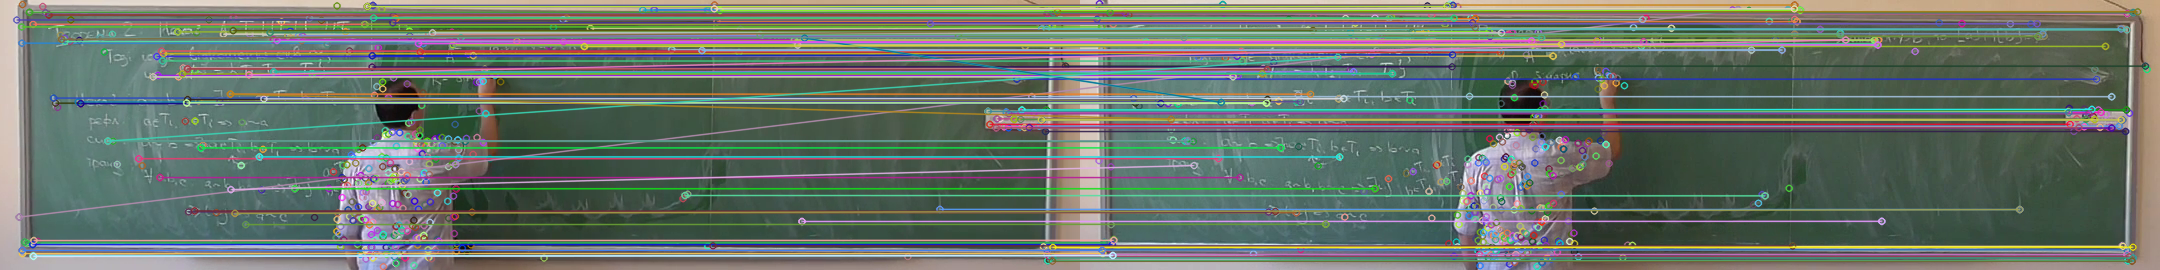
\includegraphics[width=0.55\textwidth]{images/matches_img}
    \caption{Кадри $F^i$ (верхній) та $F^{i+s}$ (нижній) із ключовими точками та лініями,
        які поєднують відповідні точки з відео \cite{yakovlev_discrete_math_video}
        \label{fig:matches_img}
    }
\end{figure}
